\chapter{Crittoanalisi}

Il \textit{principio di Kerchoffs} afferma che \textbf{la sicurezza di un sistema crittografico non deve dipendere dalla segretezza 
dell'algoritmo crittografico}, ma solo da tenerne celata la chiave. In altre parole, il sistema deve rimanere sicuro anche nell'ipotesi che il 
nemico conosca l'algoritmo di criptazione.

\noindent Esistono diverse situazioni di attacco, che corrispondono a gradi di sicurezza; più un sistema resiste a livelli di attacco alti, 
più è robusto:
\begin{itemize}
    \item \textit{Known Ciphertext Attack:} l'avversario cononosce solo il cifrato 
    \item \textit{Known Plaintext Attack:} l'avversario conosce anche il testo in chiaro 
    \item \textit{Chosen Plaintext Attack:} l'avversario può ottenere la cifratura di un testo in chiaro a sua scelta
    \item \textit{Chosen Ciphertext Attack:} l'avvversario può ottenere la decifratura di un testo cifrato a sua scelta 
    \item \textit{Chosen Text Attack:} l'avversario può ottenere la cifratura e la decifratura di coppie di testi chiaro/cifrato
\end{itemize}

$\Rightarrow$ se un cifrario viene rotto conoscendo solo il testo cifrato, allora è molto debole \dots

\section{Cifrari a shift}
Dato che prendono una lettera e la spostano di posizione, la struttura sottostante del testo rimane la stessa; in particolare, la frequenza 
delle lettere cifrate corrisponde alla frequenza delle lettere in chiaro nella lingua in cui è stato scritto il testo. 

\noindent Basta mappare le lettere fino a che viene trovata la chiave; computazionalmente parlando è molto semplice.

\section{Cifrario di Hill}

Nella sua versione standard, il cifrario di Hill è vulnerabile al \textit{\textbf{known plaintext attack}}, poiché completamente lineare: nel 
caso in cui un attaccante intercetti $n^2$ coppie chiaro-cifrato, può impostare un sistema lineare che può essere risolto. Può capitare che il 
sistema risulti indeterminato, ma è sufficiente aggiungere qualche altra coppia per renderlo risolvibile.

\noindent Per questa ragione, è richiesto poco tempo per rompere il cifrario.

\section{Cifrario di Vigenerè - Metodo Kasiski}

Il cifrario di Vigenerè resiste all'analisi delle frequenze, dato che una lettera cifrata corrisponde a più simboli in chiaro ed esiste un grande 
numero di possibli chiavi.
Un possibile attaco è il \textit{\textbf{known ciphertext attack}}, poiché permette di usare metodi statistici per individuare la lunghezza della 
chiave, per poi applicare un'analisi delle frequenze in ognuno degli alfabeti cifranti corrispondenti alle lettere della chiave.

\noindent Il metodo di Kasiski, applicabile a Vigenerè e simili, consiste nell'osservare che ci sono frequenze di caratteri identiche, poste 
ad una certa distanza di loro; questa distanza può corrispondere, con una certa probabilità, alla lunghezza della chiave o ad un suo multiplo.

\noindent Individuando tutte le sequenze ripetute (facile con un testo lungo) è probabile che la chiave sia pari al MCD tra le distanze delle 
frequenze ottenute, o un suo multiplo.

\noindent A questo punto, si può svolgere un'analisi delle frequenze.

\subsection{Indice di coincidenza}

L'indice di coincidenza di una stringa $x_1x_2\dots x_n$, rappresentato con la notazione $IC(x_1x_2\dots x_n)$, rappresenta la probabilità 
che due caratteri presi a caso nella stringa siano uguali. Lo possianmo definire come 

\begin{figure}[H]
    \centering
    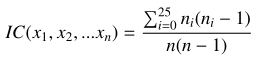
\includegraphics[width=0.4\linewidth]{chapters/chap3/images/pic1}
\end{figure}

\noindent dove $n_i$ rappresenta il numero di occorenze della $i$-esima lettera dell'alfabeto.

\noindent Con il calcolo dell'indice di coincidenza per una lettera su un testo cifrato, possiamo stabilire con quale lingua abbiamo a che fare (in 
base agli indici di coincidenza dei vari alfabeti); se vogliamo determinare la lunghezza $t$ della chiave ($t$ rappresenta il periodo
di ripetizione), possiamo procedere in questo modo:
\begin{itemize}
    \item Se $t=1$, significa che si sta usando una sostituzione monoalfabetica; posso dunque calcolare l'indice di coincidenza sul cifrato, e se ottengo 
    valori distanti da quelli delle varie lingue, posso scartare l'ipotesi di $t=1$
    \item Proseguo ipotizzando $t=2$; per poter calcolare l'$IC$, divido il mio cifrato in due sottotesti con lo shift pari a 2 $\langle(x_0x_2 \dots), (x_1x_3 \dots)\rangle$
    \item \dots
    \item Con $t=n$, si devono calcolare $n$ indici di coincidenza che avranno come caratteri quelli con uno shift pari a $n$
\end{itemize}

$\Rightarrow$ si prosegue fino a che si trovano tutti gli indici di coincidenza simili ad un indice di 
una lingua conosciuta

\begin{figure}[H]
    \centering
    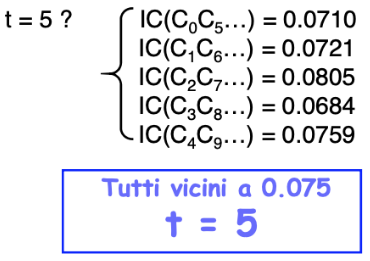
\includegraphics[width=0.5\linewidth]{chapters/chap3/images/pic2.png}
\end{figure}


\subsection{Indice mutuo di coincidenza}

Per trovare i caratteri della chiave si usa l'indice mutuo di coincidenza (IMC) che ci dice qual è la probabilità di estrarre casualmente 
da 2 stringhe 2 caratteri uguali. L'espressione che permette di calcolare IMC è 

\begin{figure}[H]
    \centering
    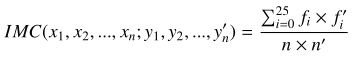
\includegraphics[width=0.6\linewidth]{chapters/chap3/images/pic3.png}
\end{figure}

\noindent dove $f_i$ rappresenta il numero di occorrenze del carattere $i$-esimo nella prima stringa, mentre $f_i^{'}$ rappresenta il numero di occorenze del 
carattere $i$-esimo nella seconda stringa.












